\chapter{T4 - Análise Bibliométrica sobre Simulação Multiagente do Dilema do Prisioneiro, por João Antonio Desidério de Moraes \label{chap:bibliometria:joaoadm94}}

\section{Introducao}
\label{MASSA@joaoadm94:introducao}


\section{Planejamento do estudo}
\label{MASSA@joaoadm94:planejamento}
\subsection{O dilema do prisioneiro}
\label{MASSA@joaoadm94:dilemadoprisioneiro}
De acordo com o verbete em \cite{noauthor_prisoners_nodate},  dilema do prisioneiro é um problema bastante conhecido no campo de teoria dos jogos e originalmente discutido por Merrill Flood e Melvin Dresher enquanto trabalhavam na RAND Corporation. 
Na descrição do dilema, dois participantes devem optar entre a cooperação ou a traição para definir o resultado da rodada. Os retornos são tais que quando ambos decidem cooperar, a recompensa é razoável para ambos; quando ambos decidem trair, a punição que recebem é igual e bem relevante. Quando discordam - um escolhe cooperar e o outro trair - o ``vencedor'' leva tudo e o ``perdedor'' tem a maior pena possível. A versão mais conhecida da narrativa do problema enuncia o seguinte:

Dois criminosos cúmplices são flagrados e presos. Após a detenção, os prisioneiros encontram-se isolados, sem possibilidade de comunicação entre si. A polícia admite ter provas para prendê-los por um delito menor mas não pelo crime principal, oferecendo então um tipo de delação premiada aos integrantes da dupla. São possíveis os seguintes resultados:

\begin{enumerate}
\item Ambos ficam em silêncio e são condenados a uma pena de 2 anos pelo delito menor;
\item Uma parte delata enquanto a outra fica em silêncio, caso em que o delator será solto e o incriminado recebe pena de 10 anos de prisão;
\item Ambos delatam um ao outro e recebem uma pena de 5 anos. 
\end{enumerate}


O formato do problema visa investigar o comportamento de participantes guiados pelos prórprios interesses em situações de conflito. Devido a sua temática de cooperação, foi aplicado na modelagem de diversos fenômenos nos campos da política e economia. A própria RAND Corporation, iniciativa onde o experimento foi desenvolvido, estudava teoria de jogos visando possíveis aplicações a estratégia nuclear global. Segundo \cite{amadae_prisoners_2016} algumas problemáticas já foram estudadas com apoio do modelo de relações do dilema do prisioneiro: controle de armas, trocas de mercado, utilização de bens públicos, mudança climática, vacinação e várias outras.

\subsection{A simulação do dilema do prisioneiro no framework MESA}
\label{MASSA@joaoadm94:simulacao}
O framework MESA, útil para modelagem e simulação do comportamento de agentes, possui uma demonstração nativa do problema do prisioneiro. A simulação consiste em uma matriz de agentes - cuja configuração inicial pode ser de cooperação ou de traição - que interagem entre si em rodadas. O retorno de cada agente em uma rodada depende das estratégias de seus vizinhos. Após iniciar a simulação, o agente adotará a estratégia do seu vizinho com maior retorno a cada iteração. Dessa forma, veremos um reforço da estratégia mais bem sucedida ao longo de toda a matriz.

Segundo a página GitHub da simulação, esse exemplo demonstra como a cooperação se torna dominante mesmo em cenários com vários agentes inicialmente traidores.

Podemos resumir o problema de interesse apresentado até agora nos seguintes termos: entender o comportamento de agentes humanos e também de agentes simulados em um ambiente de cooperação onde as condições são as mesmas propostas no famoso dilema do prisioneiro.

A simulação apresenta as seguintes variáveis independentes: 
\begin{itemize}
    \item as dimensões do campo de agentes em termos de largura e altura;
    \item o modo de escalonamento dos agentes;
    \item os pesos para cada tipo de interação.
\end{itemize}

São dependentes deles as variáveis:
\begin{itemize}
    \item a pontuação de cada agente;
    \item a última estratégia adotada pelo agente.
\end{itemize}

\subsection{Questões de pesquisa}
\label{MASSA@joaoadm94:questoes}
Visando uma pesquisa bibliométrica sobre a forma como o dilema do prisioneiro foi aplicado a pesquisas sobre diversas dinâmicas sociais, formulo as seguintes perguntas:

\begin{enumerate}
    \item Qual a base de conhecimento científico produzida sobre o tema do dilema do prisioneiro aplicado à compreensão de dinâmicas sociais de cooperação?
    \item Como o dilema do prisioneiro tem sido usado para estudar a cooperação em fenômenos sociais?
    \item Quais os principais termos e conceitos ligados à frente de pesquisa no tema de experimentos com o dilema do prisioneiro?
    \item Qual a estrutura social da comunidade que pesquisa aplicações do dilema do prisioneiro com ênfase em métodos experimentais?
\end{enumerate}

\subsection{O que já existe de pesquisa bibliométrica sobre este tema?}

\cite{glynatsi_bibliometric_2021} já fizeram um estudo bibliométrico sobre o tema. Nele foram apontados os tópicos de pesquisa e o comportamento colaborativo dos autores no campo do dilema do prisioneiro. 
Sobre os tópicos de pesquisa, cinco foram identificados: pesquisa sobre sujeitos humanos, estudos biológicos, estratégias, dinâmicas evolucionárias em redes e modelagem do dilema do prisioneiro como um jogo. O campo de pesquisa se mostra bastante colaborativo, embora a rede de co-autoria sugira existir poucas conexões diretas entre as comunidades.

\subsection{Uso do Bibliometrix e Biblioshiny}
Serão usadas a ferramenta e o \textit{workflow} proposto pelos autores do pacote Bibliometrix.

\section{Coleta de dados}
\label{joaoadm94:coleta}
Realizou-se coleta de dados usando o Web of Science no dia 10 de dezembro de 2021, acessado por meio do Portal de Periódicos da CAPES.

O acervo do Web of Science consistia nas coleções \textbf{Science  Citation  Index  Expanded (SCI -EXPANDED)} e \textbf{Social  Sciences  Citation  Index (SSCI)}, que contém registros relativos a vários campos do conhecimento. O SCI-EXPANDED foca mais na área das ciências exatas e naturais, enquanto que o SSCI indexa artigos da área das ciências sociais. Observe que os artigos nessas duas coleções são indexados desde 1945. 

Foi usada a \query\  de busca ilustrada nas linhas 1 a 9 da listagem \ref{query20221210-2}.

\lstinputlisting[numbers=left,basicstyle=\normalsize\ttfamily,caption={\query\  de busca sobre dilema do prisioneiro com ênfase em métodos experimentais.},label=query20221210-2]
{exploratory-data-analysis/joaoadm94/PesqBibliografica/PrisonerDilemma/WoS-20230128/query.txt}

\subsection{Explicação para os termos de busca usados}

A busca consistiu de quatro cláusulas disjuntivas, unidas por uma conjunção \textit{and}, aplicadas à busca por tópico.

As buscas com queries mais enxutas retornavam mais resultados. Muitos destes, entretanto, não tinham a relação desejada com o tema de simulações experimentais. Ao adicionar individualmente os outros termos constantes da query final surgiam resultados próximos do tema, mas em pequeno número. Foi preciso adicioná-los nos agrupamentos corretos para obter um número razoável de resultados interessantes à pesquisa.

\subsection{Resultados obtidos}

Os 2750 resultados obtidos na busca com os termos da query acima encontram-se no caminho ``exploratory-data-analysis/joaoadm94/PesqBibliogr/PrisonerDilemma/WoS-20221210/savedrecs.txt".

O processo de exportação dos dados ocorreu após a definição da query. O site permitia exportação de até 500 resultados em formato de texto incluindo os dados sobre citações. A pesquisa retornou mais de 2700 resultados, portanto exportou-se seis vezes, cada uma resultando em um arquivo.

A listagem \ref{record20221210} apresenta as 112 linhas de um registro no formato RIS, referentes a um artigo recuperado da Web of Science. Cada um dos campos de um registro é marcado por um código de dois caracteres, nas colunas 1 e 2 de cada linha. Se a coluna está em branco repete-se o mesmo campo da linha anterior.
O significado de cada campo pode ser visto em \citep{wikipedia_ris_2017}.

Alguns campos específicos serão comentados a seguir:
\begin{description}
    \item [PT - Publication Type] indica o tipo da publicação, no caso específico um artigo de \textit{journal} (J);
    \item [AU - Author] Nome de um autor;
    \item [AF - Author Full Name] Nome completo de um autor;
    \item [TI - Title] Título da publicação;
    \item [SO - Source] Nome da revista;
    \item [DE - Descriptor] Palavras-chave;
    \item [AB - Abstract] Resumo;
    \item [CR - Cited Referente] Cada uma das referências citadas no artigo;
    \item [TC - Times Cited] Quantidade de vezes que esse artigo foi globalmente citado;
    \item [PY - Publication Year] Ano de publicação;
    \item [VL - Volume, IS - Issue] Volume e número onde o artigo foi publicado, na revista;
    \item [BP - Begin page, EP - End page] Páginas inicial e final do artigo dentro do volume e número da revista;
    \item [DI - Digital Object Identifier] Identificador único do artigo no sistema \url{http://doi.org};
    \item [DA - Date of Acquisition] Data em que o registro foi obtido da WoS;
    \item [ER - End of Record] Fim do registro.
\end{description}

\lstinputlisting[numbers=left,basicstyle=\tiny\ttfamily,caption={Exemplo de um registro recuperado no formato RIS, sobre o tema do dilema do prisioneiro observado em redes sociais.},label=record20221210]
{exploratory-data-analysis/joaoadm94/PesqBibliografica/ris.txt}

\section{Análise dos dados}

%{\subsection{Filtra}gem de registros} - Antes da análise é possível aplicar filtros sobre os registros obtidos. Foi aplicado um filtro ao \dataset\ inicial, com 2.750 registros, que continham pŕevias de artigos, artigos de conferência, capítulos de livro etc. Foram mantidos apenas os registros de artigos publicados em revistas científicas\footnote{Assumimos as publicações em revistas como a fonte do conhecimento científico de maior qualidade.}. Após a aplicação desse filtro, foram mantidos 2.198 registros no \dataset, que será doravante chamado PrisonerDilemma/Artigos, ou MASSA@joaoadm94.

\subsection{Análise descritiva do \dataset\ MASSA@joaoadm94}

A análise bibliométrica descritiva faz uma descrição inicial do \dataset\. Para explicação detalhada de como são calculadas as diversas taxas geradas pelo Bibliometrix veja a documentação do \textit{package} a partir da página \url{https://cran.r-project.org/web/packages/bibliometrix/index.html}. A análise bibliométrica descritiva é gerada pela função \texttt{biblioAnalysis}.

As informações mais gerais sobre o \dataset\   MASSA@joaoadm94 são as seguintes:
\begin{description}
    \item [\textit{Timespan}] Os artigos resultantes da buscar e filtragem especificadas tem data de publicação entre 1962 e 2023. A base de dados tem data inicial em 1945, portanto não obtivemos resultados entre 1945 e 1961.
    \item [\textit{Sources (Journals, Books, etc)}] É 552 o número de fontes de informação que publicaram os documentos recuperados no \dataset\ MASSA@joaoadm94. Ou seja, em média, cada \textit{scientific journal} publicou $2198/552=3,9$ artigos. \footnote{Note que a média, enquanto medida de tendência central, pode não ser a que melhor reflete a tendência a quantidade de artigos publicados por revista.}
    \item [\textit{Average citations per documents}] Cada artigo no \dataset\   MASSA@joaoadm94 foi citado, em média 31,32 vezes\footnote{Note que a média, enquanto medida de tendência central, pode não ser a que melhor reflete a tendência de  citações a artigos.}.
    \item [\textit{References}] O \dataset\   MASSA@joaoadm94 contém 42.576 referências citadas (tags CR).
    \item [\textit{Keywords Plus (ID)}] 2.430 distintas palavras-chave do tipo Keywords Plus (ID)\footnote{\textit{KeyWords Plus} são ``termos de índice gerados automaticamente a partir dos títulos de artigos citados. Os termos do KeyWords Plus devem aparecer mais de uma vez na bibliografia e são ordenados de frases com várias palavras a termos únicos. O KeyWords Plus aumenta o número de resultados tradicional de palavras-chave ou títulos.'' Fonte: \url{https://images.webofknowledge.com/WOKRS410B4/help/pt_BR/WOS/hp_full_record.html}} foram encontradas no \dataset\   MASSA@joaoadm94. 
    \item [\textit{Author's Keywords (DE)}] 3.365 distintas palavras-chave indicadas pelos autores foram encontradas no \dataset\  .
    \item [\textit{Authors}] 3.902 distintos nomes de autores foram encontrados no \dataset\  \footnote{Um mesmo autor pode ter uma ou mais diferentes grafias no \dataset\  , e serão reconhecidos dois ou mais autores diferentes, embora de fato sejam apenas um. Isso significa que a quantidade de \textbf{nomes de autores} equivale à quantidade de \textbf{autores}. Adicionalmente, é possível que distintos autores sejam reconhecidos com o mesmo nome, isso é, que sejam homônimos. Ou seja, o \dataset\   em geral conterá erros de contagem na quantidade de autores reais.}.
    \item [\textit{Authors of single-authored documents}] Dentre os 3.902 distintos (nomes de) autores encontrados, 258 deles editaram artigos individualmente, isso é, sem co-autores.
    \item [\textit{Authors of multi-authored documents}] Dentre os 19.410 distintos (nomes de) autores encontrados, 3.644 deles editaram artigos com um ou mais co-autores"
    \item [\textit{Single-authored documents}] Dentre os 2.198 documentos presentes no \dataset\   MASSA@joaoadm94, 309 foram escritos por um único autor, e os restantes foram elaborados em co-autoria.
\end{description}

\subsection{Evolução da Produção Científica}

\begin{figure}
    \centering
    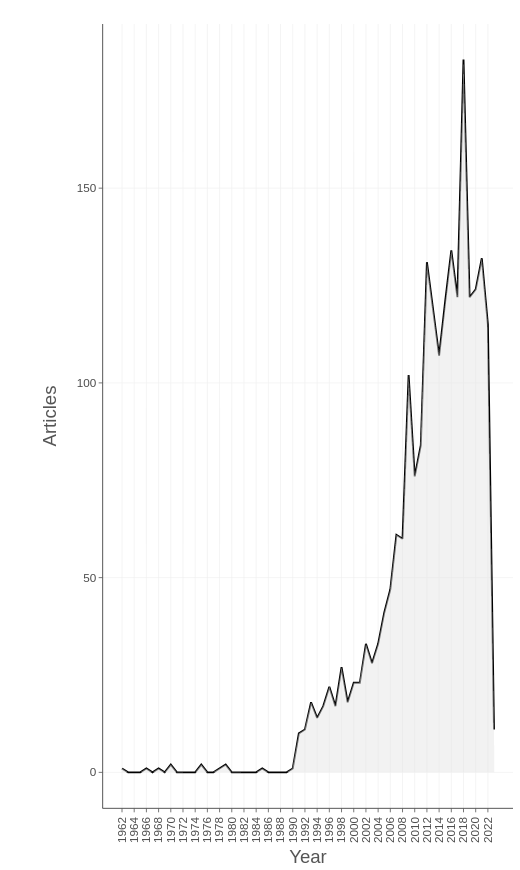
\includegraphics[height=0.5, width=1]{exploratory-data-analysis/joaoadm94/PesqBibliografica/PrisonerDilemma/WoS-20230128/Dataset/AnnualScientificProduction.png}
    \caption{Evolução da produção científica no \dataset\ MASSA@joaoadm94.}
    \label{fig:evol:anual:MASSA@joaoadm94}
\end{figure}

A figura \ref{fig:evol:anual:MASSA@joaoadm94} apresenta a evolução da produção científica mundial no tema de interesse, segundo o \dataset\   MASSA@joaoadm94. A curva mostra uma tendência de crescimento aproximadamente exponencial da quantidade de publicações a partir da década de 1990. Antes disso, a produção existe porém de forma mais tímida.

O \textit{Annual Growth Rate} do \dataset\   é de 4,01\%, próxima da taxa média de crescimento da publicação científica mundial, de cerca de 3,3\% anuais, em 2016, como ilustra o estudo em \url{https://www.researchgate.net/publication/333972683_Dynamics_of_scientific_production_in_the_world_in_Europe_and_in_France_2000-2016}, página 23.

\subsection{Interpretação do Crescimento} O acréscimo de artigos tem tendência gradual e sólida, resultando num gráfico de formato exponencial. Segundo os dados obtidos, há um pico de produção científica no ano de 2018, quando observa-se 183 artigos publicados na área. A maior taxa de crescimento do \dataset\ MASSA@joaoadm94, bem como o seu grande volume, sugerem um crescente interesse no assunto nos últimos 30 anos. 

\subsection{Evolução das Citações}

\begin{figure}
    \centering
    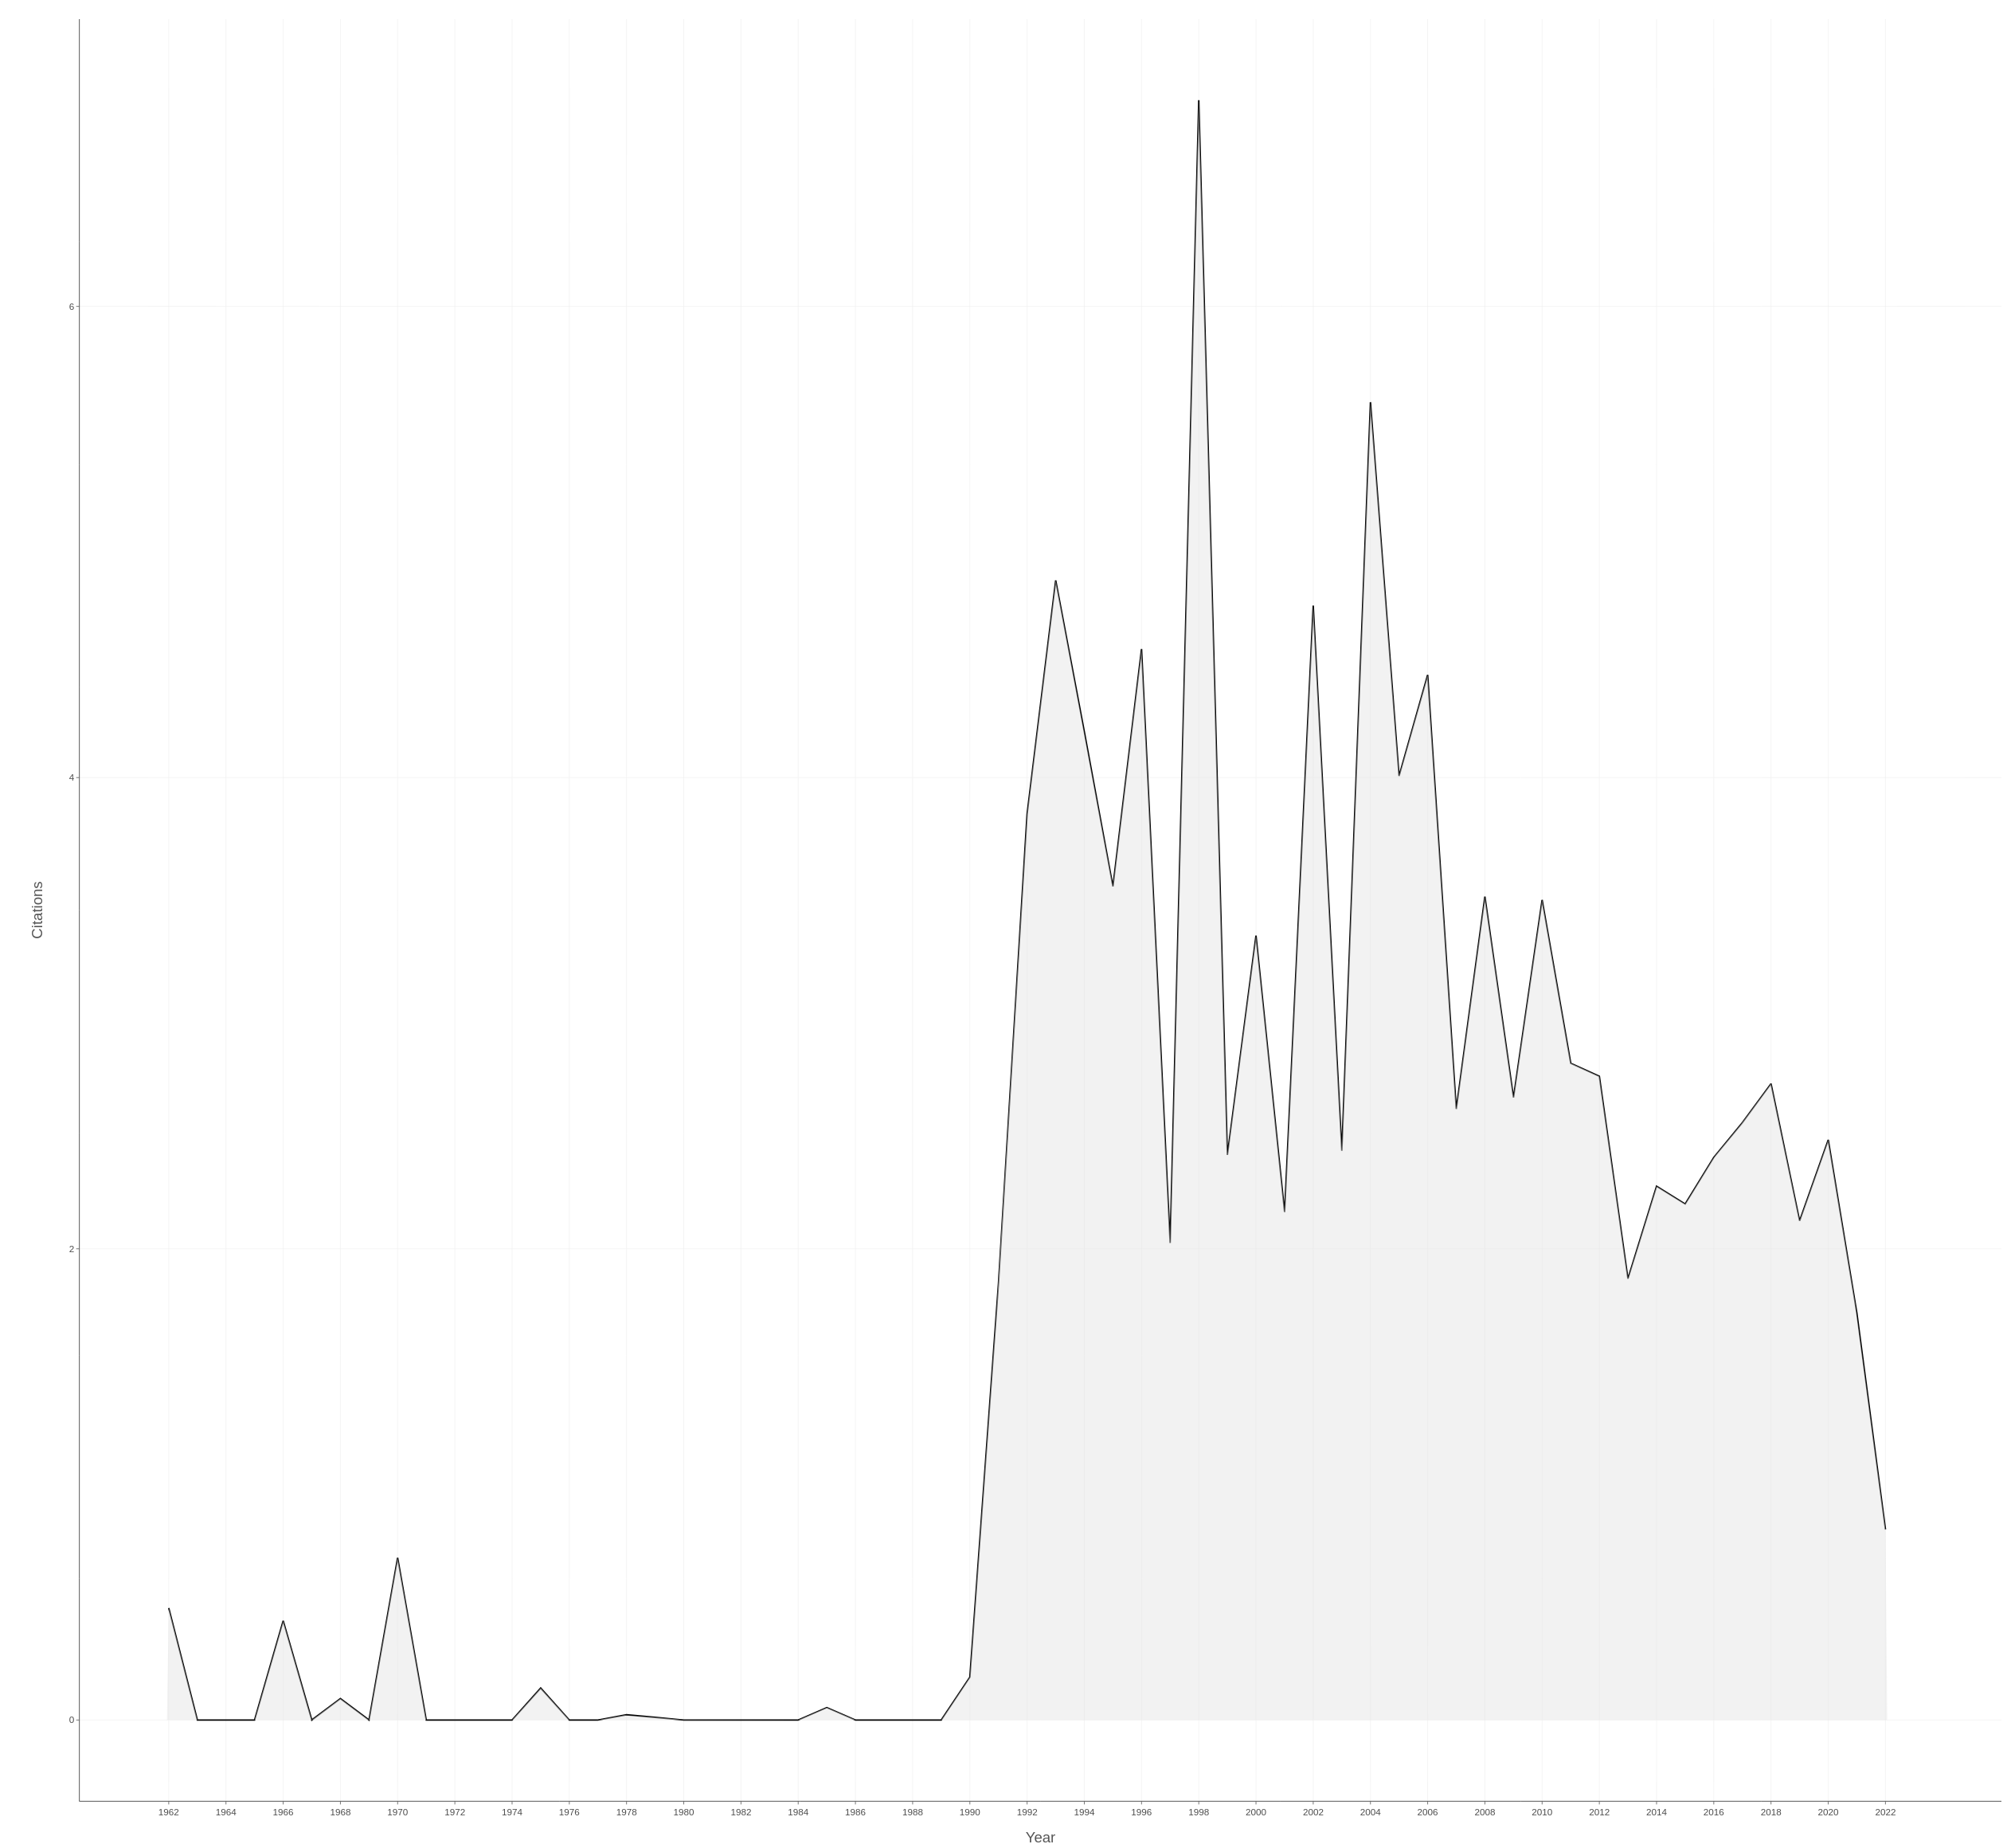
\includegraphics[width=1\textwidth]{exploratory-data-analysis/joaoadm94/PesqBibliografica/PrisonerDilemma/WoS-20230128/Dataset/AvgCitationPerYear.png}
    \caption{Evolução das citações ao \dataset\   MASSA@joaoadm94.}
    \label{fig:evol:anual:citacoes:MASSA@joaoadm94}
\end{figure}

A figura \ref{fig:evol:anual:citacoes:MASSA@joaoadm94} apresenta a evolução da média de citações aos 2.198 artigos no \dataset\   MASSA@joaoadm94. 
Nota-se variações ao longo do tempo na média anual de citações. Os artigos publicados até os anos 1990 concentram um número bem baixo de citações. Entre os anos 1990 e 2010, os artigos publicados recebem entre 2 e 6 citações por ano, período de maior efervescência dessa métrica. A partir da década de 2010, a média fica mais próxima de 2 citações. O pico que aparece no ano de 1998 deve-se, possivelmente, à presença de um artigo do \dataset, publicado em 1998, que possui um número surpreendente grande de citações. \footnote{Note que o cálculo do número  médio de citações, nesse caso, utiliza os valores computados no tag "TC (Times Cited)", já presentes no \dataset\   obtido. Ou seja, o gráfico baseia-se no número de citações globais (externas ao \dataset\   MASSA@joaoadm94), e não no número de citações locais (citações a um artigo do \dataset\ feitas por alguns dos outros artigos dentro do próprio \dataset).}.

\subsection{Interpretação das Citações}
Ao contrário do volume de publicações, o número de citações demonstra irregularidades ao longo dos anos. Isso pode sugerir que esse tema não provoque tanto interesse em cientistas de outras áreas, visto que as citações globais não acompanham o crescimento das publicações dentro do campo. Essa métrica parece sugerir que o tema possui mais relevância dentro de um nicho intelectual, carecendo ainda de aplicações úteis em outras áreas.

\subsection{\textit{Three-Field Plots (Sankey diagram)} \label{MASSA:Sankey}}

As \textit{Three-Field Plots (Sankey diagram)} (plotagens do tipo ``Três Campos'') apresentam afinidades entre três conjuntos de atributos agregados que ocorrem no \dataset. Uma plotagem do tipo Sankey busca mostrar os principais fluxos entre diferentes conjuntos de itens. \footnote{Para uma introdução ver \url{https://en.wikipedia.org/wiki/Sankey_diagram}. Para obter detalhes sobre a forma de geração e utilização desse gráfico, inclusive de forma interativa, veja o vídeo em \url{https://www.youtube.com/watch?v=jBb1iha6-sg}.} 

\begin{figure}
    \centering
    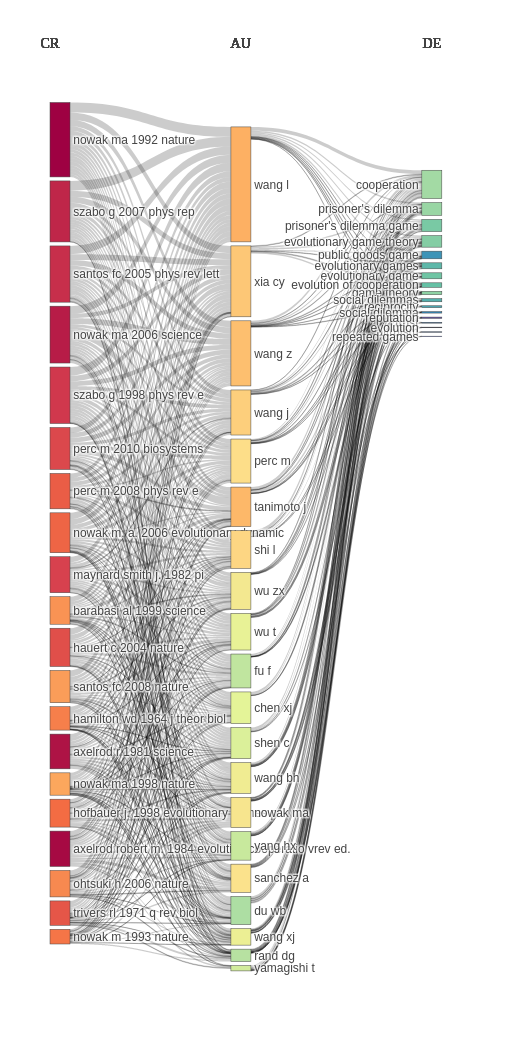
\includegraphics[scale=0.5]{exploratory-data-analysis/joaoadm94/PesqBibliografica/PrisonerDilemma/WoS-20230128/Dataset/ThreeFieldPlot-AU-CR-DE.png}
    \caption{Plotagem ``Três Campos'' (Sankey plot) do \dataset\   MASSA@joaoadm94: 20 Autores, Citações e Palavras-Chave mais proeminentes.}
    \label{fig:MASSA@joaoadm94:ThreeFieldPlot}
\end{figure}

A figura \ref{fig:MASSA@joaoadm94:ThreeFieldPlot} apresenta a plotagem do tipo ``Três Campos'' do \dataset\   MASSA@joaoadm94, vinculando, ao centro, os 20 Autores mais proeminentes (AU), à esquerda, as 20 Citações mais frequentes (CR - Cited Records), e à direita, as 20 Palavras-Chave mais frequentes empregadas pelos autores.

\subsection{Interpretação da figura \ref{fig:MASSA@joaoadm94:ThreeFieldPlot}}

Os vinte autores mais relevantes, citados pelos artigos do \dataset\ MASSA, e as palavras-chave mais relevantes são aparentemente de origem asiática, mais especificamente chinesa, com base nos sobrenomes. De outra forma, a mesma origem chinesa parece não se aplicar aos trabalhos mais citados, aparentemente europeus ou norte-americanos. Isso sugere estar ocorrendo uma migração recente da produção científica, do ocidente para o oriente. 

Adicionalmente, dentre as palavras-chave (DE) não relacionadas diretamente aos termos de busca, emergem os termos \textbf{cooperation}, \textbf{evolutionary}, \textbf{game theory} e \textbf{public goods}. Isso sugere um interesse dos autores em temas

Ainda sobre a interpretação da plotagem da figura \ref{fig:MASSA@joaoadm94:ThreeFieldPlot}, observa-se que os artigos mais citados encontram-se publicados há no mínimo mais de 13 anos atrás, sugerindo que não houve, nos últimos 13 anos, nenhum trabalho que tenha produzido uma mudança de paradigma no tema.
A fim de melhor evidenciar as citações mais relevantes segundo o peso dos autores e palavras-chave, o gráfico da figura \ref{fig:MASSA@joaoadm94:ThreeFieldPlot:10-20-20} plota apenas as 10 referências citadas, para 20 autores e palavras-chave mais proeminentes.

\begin{figure}
    \centering
    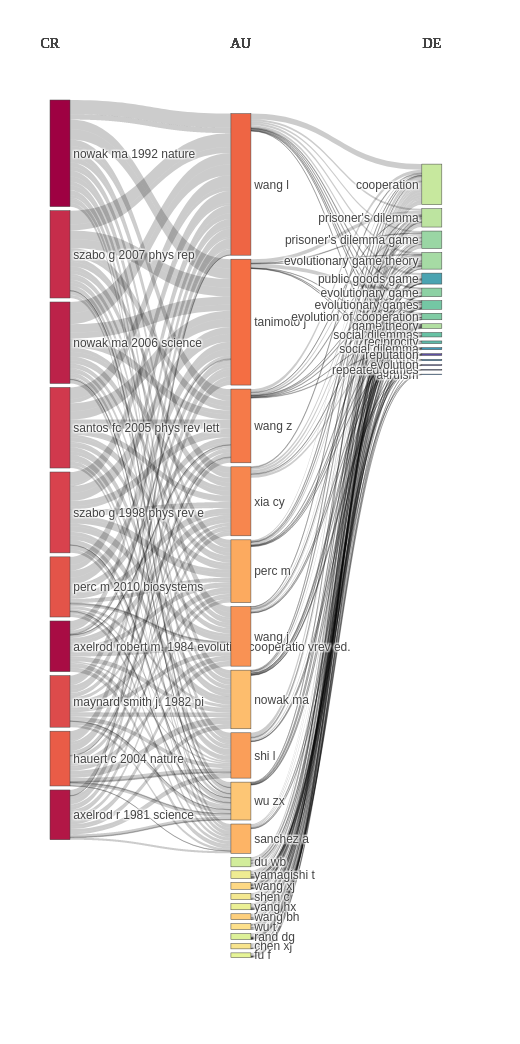
\includegraphics[height=1\textheight]{exploratory-data-analysis/joaoadm94/PesqBibliografica/PrisonerDilemma/WoS-20230128/Dataset/ThreeFieldPlot-AU-CR-DE-10-20-20.png}
    \caption{Plotagem ``Três Campos'' (Sankey plot) do \dataset\   MASSA@joaoadm94: 10 Autores, 20 Citações e Palavras-Chave mais proeminentes.}
    \label{fig:MASSA@joaoadm94:ThreeFieldPlot:10-20-20}
\end{figure}

\subsubsection{Autores mais relevantes\label{MASSA:Sankey:AutoresRelevantes}}

Breves comentários sobre cada um dos trabalhos mais citados serão apresentados a seguir.

\begin{itemize}
    \item  \cite{nowak_evolutionary_1992} explora os desdobramentos de uma simulação do dilema do prisioneiro considerando apenas dois tipos de agentes: os que sempre cooperam e os que sempre desertam;
    \item  \cite{nowak_five_2006} discute cinco mecanismos necessários à evolução da cooperação no contexto naturalmente competitivo da seleção natural biológica; 
    \item \cite{szabo_evolutionary_2006} oferece uma apresentação voltada a físicos do tema da teoria de jogos em sua forma evolucionária;
    \item \cite{santos_scale-free_2005} estuda a evolução da cooperação no arcabouço da teoria dos jogos evolucionária, adotando os dilema do prisioneiro e do amontoado de neve como metáforas de cooperação;
    \item \cite{szabo_evolutionary_1998} experimenta com um jogo simplificado de dilema do prisioneiro usando simulações Monte Carlo e técnicas de cluster dinâmico, observando as dinâmicas emergentes da variação do valor da tentação de desertar;
    \item \cite{perc_coevolutionary_2009} revisa os trabalhos recentes no tema de jogos evolucionários com incorporação de regras coevolucionárias; assim como esboça direções para estudos futuros na área;
    \item \cite{greene_review_1984} explora um modelo baseado em dilema do prisioneiro com estratégia evolucionária estável para estudar como a cooperação surge em um mundo não social, como floresce mesmo interagindo com outras estratégias e como resiste a invasão após se estabelecer; e
    \item \cite{trivers_evolution_1971} argumenta pela existência de comportamento altruísta em populações de ratos apresentando evidências para tal achado. O objetivo do estudo é propor as populações de ratos como modelo alternativo para o estudo de altruísmo e cooperação.
\end{itemize}

\subsection{Medidas bibliométricas}

As medidas bibliométricas propriamente ditas, relativas ao \dataset\ MASSA@joaoadm94, serão exploradas nesta subseção, e são organizadas em três conjuntos:
\begin{description}
    \item [Relativas às Fontes de Informação] Uma vez que foram consideradas apenas as publicações em revistas, todas as fontes de informação mensuradas serão revistas científicas, ou \textit{journals}. As principais medidas são de impacto das fontes, mensuradas com base no número de citações que os artigos publicados nas revistas obtiveram de outras publicações, possivelmente feitas em outras fontes de informação, como outras revistas, seções de livros, artigos de conferência etc. As citações são registradas pelas organizações que fazem indexação de artigos, como a Web of Science e SCOPUS;
    \item [Relativas aos Autores] Sempre que um artigo publicado por um ou mais autores e também indexado por uma organização (Web of Science,  SCOPUS etc), é citado em um outro artigo também indexado por essa mesma organização, então é feita a anotação de uma citação ao mesmo, e o impacto potencial desse autor sobre a ciência é atestado pelo valor mais alto da citação do conjunto de seus artigos indexados. Várias métricas (índice H, G, M etc) podem ser derivadas dessa medida (quantidade de citações), e são exploradas tanto em relação aos autores como em relação às revistas onde esses artigos foram publicados;
    \item [Relativas aos Documentos] Cada citação adicional a  um documento (artigo de revista, de conferência, livro, ou  capítulo de livro) é um indicador do impacto do documento em si, que evidencia a sua importância. Além das citações, a ocorrência de palavras dentro dos documentos, inclusive ordenada pelo tempo, também produz indicadores numéricos (métricas) relevantes para analisar a importância do documento em relação a outros. 
\end{description}

Essas medidas serão apresentadas a seguir.

\subsubsection{Bibliometrias aplicadas aos documentos (Artigos científicos) no \dataset}

\paragraph{Citações globais aos artigos no \dataset}

Cada registro recuperado no \dataset\ apresenta um conjunto de informações, dentre as quais pode constar a quantidade de vezes que uma citação ao mesmo foi registrada no índice do WoS, desde que no momento da extração seja feita essa solicitação (\textit{TC - Times Cited}).
A tabela \ref{tab:MASSA:GlobalCitations} apresenta a lista dos 25 artigos do \dataset, que foram mais citados, ordenados de forma decrescente pelo número global de citações do artigo, nos índices da WoS. Para cada artigo é apresentada a referencia abreviada, o DOI e a quantidade de vezes que ele foi citado globalmente (no índice do WoS). Para recuperar a página do artigo deve-se abrir uma url prefixada com \url{http://doi.org/}, e informar o valor do DOI indicado, por exemplo \url{http://doi.org/10.1257/jel.47.2.448} levará à página do artigo mais citado, cujo título é ``Gender Differences in Preferences'.

\begin{table}[htp]
    \centering
\footnotesize
\csvreader[tabular = |r|l|l|r|,
separator=semicolon
%,filter not strcmp={\csvcolii}{},
, table head = \hline\hline \# & Artigo (Referência Abreviada) & DOI (Digital Object Identifier) & Tot.Cit.\\ \hline\hline,
table foot = \hline\hline
]{exploratory-data-analysis/joaoadm94/PesqBibliografica/PrisonerDilemma/WoS-20230128/Metricas/Most_Global_Cited_Documents.csv}
{Paper=\paper, DOI=\doi,Total Citations=\totcit}
{ \thecsvrow & {\tiny\paper} & {\tiny \doi} & \totcit}
    \caption{25 artigos mais citados globalmente no \dataset\ MASSA@joaoadm94.}
    \label{tab:MASSA:GlobalCitations}
\end{table}

Após a visitação do resumo do texto de vários dos documentos citados, percebe-se que não refletem bem o foco do \dataset, o que se justifica pelo fato de que esses documentos são os de maior citação global. Isso significa que  e não necessariamente os que tem maior citação local ao \dataset. Dessa forma, procede-se à próxima análise.

\paragraph{Citações locais aos artigos no \dataset}

Cada registro recuperado no \dataset\ apresenta um conjunto de informações, dentre as quais consta a lista das citações feitas a outros documentos, nas seção bibliografia. O Bibliometrix computa de forma aproximada a quantidade de vezes que cada artigo do \dataset\ foi citado por outros artigos do mesmo \dataset, construindo uma tabela das maiores citações locais, que provavelmente apontará para artigos com afinidade bem maior à busca efetuada.

\begin{table}[htp]
    \centering
\footnotesize
\csvreader[tabular = |r|l|l|r|r|,
separator=semicolon,
% filter not strcmp={\csvcolii}{},
table head = \hline\hline \# & Artigo (Referência Abreviada) & DOI  & L.Cit & G.Cit\\ \hline\hline,
table foot = \hline\hline
]{exploratory-data-analysis/joaoadm94/PesqBibliografica/PrisonerDilemma/WoS-20230128/Metricas/Most_Local_Cited_Documents.csv}
{Document=\paper,DOI=\doi}
{\thecsvrow & {\tiny\paper} & {\tiny\doi} & \csvcoliii & \csvcoliv}
    \caption{25 artigos mais citados localmente no \dataset\ MASSA@joaoadm94.}
    \label{tab:MASSA:LocalCitations}
\end{table}

A lista dos artigos retornados pelo critério de citação local retornou textos bastante pertinentes ao tema da simulação multiagente de fenômenos sociais, conforme os 10 títulos a seguir listados, seguindo a ordem apresentada na tabela:
\begin{enumerate}
    \item ``Evolutionary games on graphs'' oferece uma apresentação voltada a físicos do tema da teoria de jogos em sua forma evolucionária;%\footnote{\textit{Game theory is one of the key paradigms behind many scientific disciplines from biology to behavioral sciences to economics. In its evolutionary form and especially when the interacting agents are linked in a specific social network the underlying solution concepts and methods are very similar to those applied in non-equilibrium statistical physics. This review gives a tutorial-type overview of the field for physicists. The first four sections introduce the necessary background in classical and evolutionary game theory from the basic definitions to the most important results. The fifth section surveys the topological complications implied by non-mean-field-type social network structures in general. The next three sections discuss in detail the dynamic behavior of three prominent classes of models: the Prisoner's Dilemma, the Rock–Scissors–Paper game, and Competing Associations. The major theme of the review is in what sense and how the graph structure of interactions can modify and enrich the picture of long term behavioral patterns emerging in evolutionary games.}};
    \item ``Evolutionary prisoner’s dilemma game on a square lattice'' explora os desdobramentos de uma simulação do dilema do prisioneiro considerando apenas dois tipos de agentes: os que sempre cooperam e os que sempre desertam;%\footnote{\textit{A simplified prisoner’s game is studied on a square lattice when the players interacting with their neighbors can follow two strategies: to cooperate (C) or to defect (D) unconditionally. The players updated in random sequence have a chance to adopt one of the neighboring strategies with a probability depending on the payoff difference. Using Monte Carlo simulations and dynamical cluster techniques, we study the density c of cooperators in the stationary state. This system exhibits a continuous transition between the two absorbing states when varying the value of temptation to defect. In the limits →c0 and 1 we have observed critical transitions belonging to the universality class of directed percolation.}};
    \item ``Spatial structure often inhibits the evolution of cooperation in the snowdrift game'' estuda o impacto da estrutura espacial na evolução da estratégia cooperativa em simulações do modelo snowdrift;%\footnote{\textit{Understanding the emergence of cooperation is a fundamental problem in evolutionary biology. Evolutionary game theory has become a powerful framework with which to investigate this problem. Two simple games have attracted most attention in theoretical and experimental studies: the Prisoner's Dilemma and the snowdrift game (also known as the hawk–dove or chicken game). In the Prisoner's Dilemma, the non-cooperative state is evolutionarily stable, which has inspired numerous investigations of suitable extensions that enable cooperative behaviour to persist. In particular, on the basis of spatial extensions of the Prisoner's Dilemma, it is widely accepted that spatial structure promotes the evolution of cooperation. Here we show that no such general predictions can be made for the effects of spatial structure in the snowdrift game. In unstructured snowdrift games, intermediate levels of cooperation persist. Unexpectedly, spatial structure reduces the proportion of cooperators for a wide range of parameters. In particular, spatial structure eliminates cooperation if the cost-to-benefit ratio of cooperation is high. Our results caution against the common belief that spatial structure is necessarily beneficial for cooperative behaviour.}};
\item ``A strategy of win-stay, lose-shift that outperforms tit-for-tat in the Prisoner's Dilemma game'' avalia o sucesso de estratégias alternativas ao toma-lá-dá-cá em simulações do dilema do prisioneiro;%\footnote{\textit{The Prisoner's Dilemma is the leading metaphor for the evolution of cooperative behaviour in populations of selfish agents, especially since the well-known computer tournaments of Axelrod and their application to biological communities. In Axelrod's simulations, the simple strategy tit-for-tat did outstandingly well and subsequently became the major paradigm for reciprocal altruism. Here we present extended evolutionary simulations of heterogeneous ensembles of probabilistic strategies including mutation and selection, and report the unexpected success of another protagonist: Pavlov. This strategy is as simple as tit-for-tat and embodies the fundamental behavioural mechanism win-stay, lose-shift, which seems to be a widespread rule. Pavlov's success is based on two important advantages over tit-for-tat: it can correct occasional mistakes and exploit unconditional cooperators. This second feature prevents Pavlov populations from being undermined by unconditional cooperators, which in turn invite defectors. Pavlov seems to be more robust than tit-for-tat, suggesting that cooperative behaviour in natural situations may often be based on win-stay, lose-shift.}};
\item ``Evolution of indirect reciprocity by image scoring'' tenta demonstrar a estabilidade da reciprocidade indireta como mecanismo evolutivo em simulações de cenários de competitividade ;%\footnote{\textit{Darwinian evolution has to provide an explanation for cooperative behaviour. Theories of cooperation are based on kin selection (dependent on genetic relatedness), group selection and reciprocal altruism. The idea of reciprocal altruism usually involves direct reciprocity: repeated encounters between the same individuals allow for the return of an altruistic act by the recipient. Here we present a new theoretical framework, which is based on indirect reciprocity and does not require the same two individuals ever to meet again. Individual selection can nevertheless favour cooperative strategies directed towards recipients that have helped others in the past. Cooperation pays because it confers the image of a valuable community member to the cooperating individual. We present computer simulations and analytic models that specify the conditions required for evolutionary stability of indirect reciprocity. We show that the probability of knowing the ‘image’ of the recipient must exceed the cost-to-benefit ratio of the altruistic act. We propose that the emergence of indirect reciprocity was a decisive step for the evolution of human societies.}};
\item ``Models of cooperation based on the Prisoner’s
Dilemma and the Snowdrift game'' examina o impacto de extensões e modificações nas variáveis independentes dos modelos "dilema do prisioneiro" e pelo "jogo do amontoado de neve";%\footnote{\textit{Understanding the mechanisms that can lead to the evolution of cooperation through natural selection is a core problem in biology. Among the various attempts at constructing a theory of cooperation, game theory has played a central role. Here, we review models of cooperation that are based on two simple games: the Prisoner’s Dilemma, and the Snowdrift game. Both games are two-person games with two strategies, to cooperate and to defect, and both games are social dilemmas. In social dilemmas, cooperation is prone to exploitation by defectors, and the average payoff in populations at evolutionary equilibrium is lower than it would be in populations consisting of only cooperators. The difference between the games is that cooperation is not maintained in the Prisoner’s Dilemma, but persists in the Snowdrift game at an intermediate frequency. As a consequence, insights gained from studying extensions of the two games differ substantially. We review the most salient results obtained from extensions such as iteration, spatial structure, continuously variable cooperative investments, and multi-person interactions. Bridging the gap between theoretical and empirical research is one of the main challenges for future studies of cooperation, and we conclude by pointing out a number of promising natural systems in which the theory can be tested experimentally.}};
\item ``Statistical physics of human cooperation'' compara as estatísticas obtidas em modelos tradicionais de interação entre partículas com aqueles obtidos em modelos de interação social como o dilema do prisioneiro;%\footnote{\textit{Extensive cooperation among unrelated individuals is unique to humans, who often sacrifice personal benefits for the common good and work together to achieve what they are unable to execute alone. The evolutionary success of our species is indeed due, to a large degree, to our unparalleled other-regarding abilities. Yet, a comprehensive understanding of human cooperation remains a formidable challenge. Recent research in the social sciences indicates that it is important to focus on the collective behavior that emerges as the result of the interactions among individuals, groups, and even societies. Non-equilibrium statistical physics, in particular Monte Carlo methods and the theory of collective behavior of interacting particles near phase transition points, has proven to be very valuable for understanding counterintuitive evolutionary outcomes. By treating models of human cooperation as classical spin models, a physicist can draw on familiar settings from statistical physics. However, unlike pairwise interactions among particles that typically govern solid-state physics systems, interactions among humans often involve group interactions, and they also involve a larger number of possible states even for the most simplified description of reality. The complexity of solutions therefore often surpasses that observed in physical systems. Here we review experimental and theoretical research that advances our understanding of human cooperation, focusing on spatial pattern formation, on the spatiotemporal dynamics of observed solutions, and on self-organization that may either promote or hinder socially favorable states.}};
\item ``Evolutionary game theory: Temporal and spatial effects beyond replicator dynamics'' explora os limites explicativos da equação replicadora aplicada a modelos de teoria dos jogos no contexto de outras disciplinas;%\footnote{\textit{Evolutionary game dynamics is one of the most fruitful frameworks for studying evolution in different disciplines, from Biology to Economics. Within this context, the approach of choice for many researchers is the so-called replicator equation, that describes mathematically the idea that those individuals performing better have more offspring and thus their frequency in the population grows. While very many interesting results have been obtained with this equation in the three decades elapsed since it was first proposed, it is important to realize the limits of its applicability. One particularly relevant issue in this respect is that of non-mean-field effects, that may arise from temporal fluctuations or from spatial correlations, both neglected in the replicator equation. This review discusses these temporal and spatial effects focusing on the non-trivial modifications they induce when compared to the outcome of replicator dynamics. Alongside this question, the hypothesis of linearity and its relation to the choice of the rule for strategy update is also analyzed. The discussion is presented in terms of the emergence of cooperation, as one of the current key problems in Biology and in other disciplines.}};
\item ``Phase diagrams for an evolutionary prisoner’s dilemma game on two-dimensional lattices'' experimenta com um jogo simplificado de dilema do prisioneiro usando simulações Monte Carlo e técnicas de cluster dinâmico, observando as dinâmicas emergentes da variação do valor da tentação de desertar;%\footnote{\textit{The effects of payoffs and noise on the maintenance of cooperative behavior are studied in an evolutionary prisoner’s dilemma game with players located on the sites of different two-dimensional lattices. This system exhibits a phase transition from a mixed state of cooperators and defectors to a homogeneous one where only the defectors remain alive. Using Monte Carlo simulations and the generalized mean-field approximations we have determined the phase boundaries (critical points) separating the two phases on the plane of the temperature (noise) and temptation to choose defection. In the zero temperature limit the cooperation can be sustained only for those connectivity structures where three-site clique percolation occurs.}};
\item ``Promotion of cooperation induced by appropriate payoff aspirations in a small-world networked game'' investiga a contribuição do fator aspiracional para o surgimento e manutenção da cooperação em dinâmicas sociais;%\footnote{\textit{Based on learning theory, we adopt a stochastic learning updating rule to investigate the evolution of cooperation in the Prisoner’s Dilemma game on Newman-Watts small-world networks with different payoff aspiration levels. Interestingly, simulation results show that the mechanism of intermediate aspiration promoting cooperation resembles a resonancelike behavior, and there exists a ping-pong vibration of cooperation for large payoff aspiration. To explain the nontrivial dependence of the cooperation level on the aspiration level, we investigate the fractions of links, provide analytical results of the cooperation level, and find that the simulation results are in close agreement with analytical ones. Our work may be helpful in understanding the cooperative behavior induced by the aspiration level in society.}};
\item ``Towards effective payoffs in the prisoner’s dilemma game on scale-free networks'' pesquisa técnicas de normalização dos prêmios do dilema do prisioneiro em redes de agentes livres de escala ;%\footnote{\textit{We study the transition towards effective payoffs in the prisoner’s dilemma game on scale-free networks by introducing a normalization parameter guiding the system from accumulated payoffs to payoffs normalized with the connectivity of each agent. We show that during this transition the heterogeneity-based ability of scale-free networks to facilitate cooperative behavior deteriorates continuously, eventually collapsing with the results obtained on regular graphs. The strategy donations and adaptation probabilities of agents with different connectivities are studied. Results reveal that strategies generally spread from agents with larger towards agents with smaller degree. However, this strategy adoption flow reverses sharply in the fully normalized payoff limit. Surprisingly, cooperators occupy the hubs even if the averaged cooperation level due to partly normalized payoffs is moderate.}};
\end{enumerate}
